\chapter{Design and Methodology}


\begin{center}
\begin{table}
\centering
\begin{tabular}{ | c | c |}
 \hline
 \textbf{Devices} & \textbf{Requirements} \\ 
 \hline \hline
 Processor & Any Updated Processor \\ 
 RAM & Min 4GB \\  
 Hard Disk & Min 100 GB \\    
 \hline
\end{tabular}
\caption{Hardware Requirements}
\end{table}
\end{center}

\begin{center}
\begin{table}
\centering
\begin{tabular}{ | c | c |}
 \hline
 \textbf{Type} & \textbf{System} \\ 
 \hline \hline
 Operating System & Any Updated Processor \\ 
 Technology & Python3.6 \\  
 IDE & PyCharm \\    
 Front End & PyQt5 \\
 Operating System & Windows \\

 \hline
\end{tabular}
\caption{Software Requirements}
\end{table}
\end{center}


\section{System Analysis}
\subsection{What is a Waterfall Model?}
The Waterfall Model is a phase-by-phase method for partitioning software development. Each step of the SDLC is designed to be used for specialised tasks. Winston Royce was the first to debut it in 1970.
\subsection{Requirements:}
The first stage entails determining what needs to be created, as well as the function and purpose of the structure. The specs of the product, as well as its inputs and outputs, are checked and reported here.
\subsection{System design}
This step evaluates the requirements from the first phase and creates the system design. The system design aids in the selection of hardware and software, as well as the overall system architecture. The software code for the next level is currently being written.

\subsection{Implementation}
The system is built up of smaller programmes called devices, each with its own set of system design inputs, which are then integrated in the following phase. Unit testing is the process of creating and testing each unit's functionality.
\subsection{Inclusion and Testing}
All of the units developed during the implementation phase are incorporated into the system after each item has been tested. To uncover any problems or challenges, the application must be tested on a regular basis. Tests are conducted to ensure that the consumer has no difficulties installing the programme.
\subsection{Deployement of the System}
The product is deployed or supplied to the customer once functional and non-functional testing is completed.

After the system or component has been installed, changes are needed to improve or boost performance. These changes could be made in response to client requests or as a consequence of issues that arise while the system is in use. Ongoing software support and maintenance are offered to the customer.


\section{Rights of Functioning}

\begin{itemize}
\item Login as an Adminstrator
\item Add a photo to your profile
\item  Detecting Plant Disease
\item Precognition
\item Training and Education
\item Image Analysis 
\item Results of the Image
\end{itemize}

\section{Non-Functional Requirements}
\subsection{What is Non Functional Requirement?}
NON-FUNCTIONAL REQUIREMENT (NFR) is a quality indicator for software systems. They evaluate the software system's responsiveness, usability, security, portability, and other features, all of which are crucial to its success. A non-functional request would be, "How fast does the site charge?" Systems that do not meet user requirements may arise if non-functional criteria are not used.
Non-functional criteria can be used to constrain or limit the design of a system across multiple agile backlogs. If the number of visitors to the site exceeds 10,000, the website should load in three seconds. Non-functional needs are just as significant as functional requirements.

\subsection{Examples of Non Functional Requirements}
\begin{enumerate}
\item After the first successful login, users must update the previously set login password. In addition, the beginning must never be repeated.
\item Employees demanded that their pay information be updated. The security administrator should be notified about this attempt.
\item For each unsuccessful user attempt to access the data item, an audit trail is kept.
\item A website should be able to track the activity of 20 million people at the same time.
\item  Is software portability required? As a result, switching between operating systems isn't a problem.
\item Information confidentiality, technological export limits, intellectual property rights, and other issues should all be looked into.
\end{enumerate}

\subsection{Benefits of Non Functional Requirements}

\begin{itemize}
\item They offer a fantastic user experience and straightforward software deployment.
\item They assist in the development of a software security policy. 
\end{itemize}

\subsection{Drawbacks of Non Functional Requirements}
\begin{itemize}
\item The high-quality software subsystems are unaffected by any functional requirement.
\item Extra attention is necessary throughout the software architecture / high-level design phase, which increases costs.
\item When they're implemented, they normally don't result in the establishment of a new software subsystem.
\item It's difficult to change non-functional items after the architectural phase is finished.
\end{itemize}

\section{Implementation}

The original data set was increased offline to create this data set. The original dataset is included in this project. This dataset contains roughly 87K pictures of healthy and damaged crop leaves divided into 38 classifications. To preserve the directory's structure, the complete data set is split into 80/20 training and validation ratios. A fresh directory with 33 test images will be released later.

Convolution covnets, or computational neural networks, are neural networks with shared parameters.

Layers are classified as follows:

\begin{enumerate}
\item The input layer
\item Convolutional Layer
\item The Layers' Activation
\item The layer of a swimming pool
\item A layer that is completely connected
\end{enumerate}

\begin{figure}[]
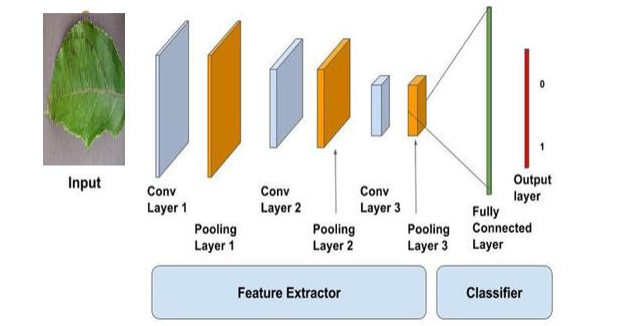
\includegraphics{Capture}
\caption{CNN Layer}
\end{figure}

The image's raw input is stored on this layer, which has a width of 32 pixels, a height of 32 pixels, and a depth of three pixels.
The output volume is computed by computing the dot product between all filters and the image patch in the convolution layer. This layer's output volume will be 32 × 32 x 12 if we use a total of 12 filters.

This layer will apply an element-by-element activation function to the output of the convolution layer. Frequent activation functions include RELU:max(0,x),Sigmoid: $\frac{1}{1+e^{-x}}$
